\documentclass[letter, 12pt]{article}
\usepackage{comment} % enables the use of multi-line comments (\ifx \fi) 
\usepackage{lipsum} %This package just generates Lorem Ipsum filler text. 
\usepackage{fullpage} % changes the margin
\usepackage[headsep=1cm, margin=1in]{geometry}
\usepackage{amsmath,amsthm,amssymb,amsfonts} %math packages
\usepackage{enumitem}
\usepackage[mathscr]{euscript}
\usepackage{accents}
\usepackage{units}
\usepackage{listings}
\usepackage{titlesec}
\usepackage{braket}
\usepackage{slashed}
\usepackage{graphicx} %graphics
\usepackage{breqn}
\usepackage{array}
\usepackage{multicol}
\usepackage{hyperref}
\usepackage{indentfirst}
\usepackage{fancyhdr}
\usepackage[none]{hyphenat} 
\usepackage{color}
\usepackage[draft]{todonotes}
%\usepackage[disable]{todonotes}
\usepackage{tikz-cd}
\usepackage{setspace}
\usepackage{colortbl}


%\renewcommand{\baselinestretch}{1.0} 
%\titlespacing*{<command>}{<left>}{<before-sep>}{<after-sep>}
%\titlespacing{\section}
%{0pt}{0pt}{1pt}
%\titlespacing{\subsection}
%{0pt}{0pt}{1pt}



% bibliography packages
\usepackage{natbib}
\bibpunct{(}{)}{;}{a}{}{,}
\bibliographystyle{apsr}
% dcolumn package: table
%\usepackage{dcolumn}
%\newcolumntype{.}{D{.}{.}{-1}}
%\newcolumntype{d}[1]{D{.}{.}{#1}}

% Title 
\title{Franchise, Inequality and US State Income Tax Adoption}
\titleformat{\subsection}[runin]
{\normalfont\large\bfseries}{\thesubsection}{1em}{}
\author{Moratz, Donald \thanks{Authors names are in alphabetical order.}\thanks{This version of the paper is presented by Donald Moratz for the purpose of the final paper for Maximum Likelihood} \and Cheung, Gloria \and Holmes, David}
\date{Last compiled: April 30, 2018}

%\pagestyle{fancy}
%\fancyhf{}
%\rhead{Cheung}
%\lhead{Econ 750: Midterm Review}
%\rfoot{Page \thepage}

\pagestyle{fancy}
\fancyhf{}
\fancyhead[L]{}
\fancyhead[R]{Cheung, Holmes, Moratz | p \thepage}



\begin{document} 

\thispagestyle{plain}
\maketitle	

\begin{abstract}
	This paper examines the state-level adoption of income taxes in the United States following the federal level adoption of the income tax in 1913. States exhibit substantial variation in adoption over a period of around six decades that is unexplained in the current literature surrounding the adoption of the income tax at the federal level. Using historical agricultural census data and U.S. general census data, we created an original time-series dataset ranging from 1900 to 1974 that measures heretofore proposed factors influencing the adoption of income tax at the federal level. We propose several hypotheses around the factors that influence the adoption of the income tax- placing new emphasis on within state variation- while still controlling for national level shocks, such as war and the Great Depression. We posit that inequality is a primary driver of the adoption of the income tax, and that it works, at least partially, through the extension of franchise as a causal mechanism. We find support for our argument by using causal mediation in a binary logistic regression model. 
\end{abstract}

\pagebreak

%intro, lit review, historical perspective/data collection, theoretical argument, method of analysis and description of results, conclusion

\doublespacing


\section{Introduction}

The modern state is frequently defined by its capacity to assert control over its borders and its citizens. Whether this control is related to its geographic sanctity, internal sovereignty, or its fiscal capacity, significant analysis has been done attempting to measure a state’s ability to govern (\citealt{hendrix2010measuring}, \citealt{hanson2013leviathan}, \citealt{ottervik2013conceptualizing}, \citealt{berry1997measuring}, and many others). Since a key component of state capacity derives from its ability to fund its activities, a small segment of scholarship has arisen within political science studying taxation.  Much of the existing work on the income tax - a key source of revenue for many states - portrays the centrality of the tax administration as a tool that enabled the state to expand and take on a greater diversity of roles in the lives of its citizens. Indeed, the income tax is of particularly critical importance given the evidence that developing states that better operationalize it tend to have higher levels of growth (\citealt{moore2004revenues}). Explanations that combine the political and economic considerations that influence the implementation of the income tax have focused attention on elites serving either as obstacles to income tax adoption, or under the right conditions, as amenable or even primary drivers for the creation of tax administration apparatuses (\citealt{mares2015non}).

The current political economy literature primarily examines the incidence of the income tax through a comparative perspective, focusing on its adoption on a national level by different governments. We propose instead that examining states within federal systems is a better test of political conditions due to the heterogeneity of the international system. An excellent case study is the United States, which has well defined intrastate borders, institutionally strong local governments, and had a wide dispersion in the rates of adoption across states.  In the case of the United States, we argue that variation in the timing of individual state governments in adopting the income tax reflects differences in the political environments that conditions the choices of elites and legislators.

While significant work has been done on the adoption of the income tax at the national level (\citealt{mares2015non}; \citealt{ardanaz2013inequality}; \citealt{beramendi2014electoral}; \citealt{scheve2010conscription}), less work has been done on understanding what drives the implementation at the sub-national level. By examining the historical instances of adoption in the United States, we identify trends that merit further explanation and uncover interesting discrepancies within the current literature suggesting that, at least within the United States, there exists potential for further examination beyond the current theories proposed by extant literature.

In this paper, we are engaging with the current literature surrounding income tax adoption, examining the historical context of taxation within the United States, and proposing several new hypotheses on the driving forces of income taxation adoption. We focus on the relationship between rural inequality, franchise and the adoption of the income tax. Using a measure of urbanization, we examine the impact of changing geographic population distribution and the continued development of an industrialized economy. A key component of the history of our sample concerns distinct time periods: the pre-Great Depression era, the Great Depression and World War II era, and the post-World War II era. These eras create cleavages that stretch the current narratives of income tax adoption and require an expansion of alternative, plausible explanations. We find that at the very least, the Great Depression period is distinct in a consistent way that fundamentally altered the political structure and increased the likelihood of adoption of the income tax. We attempt to build a unified theory around the adoption of the income tax that extends the current understanding of contemporary literature. As we examine the historical rates of adoption, a pattern emerges in our historical analysis: that state-level income tax adoption tended to cluster in time, and that these clusters correspond with changes in society - the most noteworthy of which is the onset of the Great Depression. Accounting for these factors reveals a new theory around income tax adoption that is an extension of, and in some ways a challenge to current literature. 

Furthermore, we will provide empirical evidence to support our key hypotheses. First, we argue that rural inequality is negatively related to the adoption of the income tax. Second, increasing urbanization decreased the likelihood of a state adopting the income tax. Third, that the largest proponents of income tax adoption were a strong agrarian middle class, rather than agrarian elites, so that income tax adoption was most likely with middle levels of rural inequality. Fourth, that preferences regarding spending affected the adoption of the income tax - most notably, as demand for state spending rose during the Great Depression, the likelihood governing the expansion of the income tax had a statistically significant increase. Fifth, low levels of the franchise does indeed increase the likelihood of income tax adoption. Finally, we argue that franchise primarily serves as a mechanism through which rural inequality operates to affect the adoption of the income tax, rather than as an underlying cause in and of itself.

The paper will proceed in the following sections. Section 2 will undertake an examination of the current literature to motivate our baseline model. Section 3 undertakes a historical review of taxation- as well as other societal changes- within the United States- both its implementation and development over time at the federal and subnational level. Section 4 develops our theory and provides hypotheses that we will test using several empirical models. Section 5 provides a summary of the data we use, including descriptive statistics to characterize our sample set. Section 6 introduces our method of analysis - primarily logistic regressions - to test several of our key hypotheses. Section 7 undertakes a causal mediation examination to test our final hypothesis surrounding the impact of franchise as a mechanism through which rural inequality operates to affect the adoption of the income tax.  Section 8 will examine several robustness checks. Finally, Section 9 concludes and provides areas for additional future research.


\section{Taxation and the State}

This section seeks to conduct a review of some of the literature surrounding the development of taxation at the national level. We begin first with the history and causes behind the creation of the fiscal state. Recognizing that these explanations are limited in explaining subnational developments, we move into a discussion of the literature surrounding elites and the role of distributional conflicts in influencing the taxation. This literature, while still primarily focused on the national level, suggests an alternative, plausible mechanisms by which sub-national bureaucratic organizations develop and the adoption of the income tax takes place.

\subsection{Development of State Capacity}\hfill\\

The income tax as an instrument of the state's fiscal extractive capacity fundamentally grounds its analysis on the level of state-based comparisons. Historically, the development of the fiscal state was stunted by the concentration of economic and political power amongst a select group of elites. This, in turn, reduced the incentives of those in power to invest in state capacity. Collecting a wider expanse of taxes necessitated increasing the bureaucratic and administrative capacities of government (\citealt{cardenas2010state}). However, these increases also lead to a subsequent dispersion of power from a centralized elite into various sectors of the government.

Therefore, a burgeoning question in the political economy literature is how the fiscal state emerged – a predominant school of thought points to the importance of warfare, which encouraged fiscal innovation and subsequent expansion by states. A related body of literature also relates warfare to state formation (\citealt{tilly1992coercion}), though it is not our central focus. The expansion of state capacity was a rational response to exogenous pressure, \cite{scheve2010conscription}, the relationship between warfare and modern fiscal institutions is one that is oft-explored in the literature (\citealt{dincecco2012warfare}; \citealt{besley2009origins}).

Yet such a view of the development of fiscal capacity not only fails to explain the adoption of fiscal institutions in states that have not faced the threat of war or political conflict; the above outlined narrative might also unfold quite differently in federalist states - where the adoption of the income tax on the federal level does not guarantee a parallel adoption at the state level. The potential for the income tax to serve as a mechanism of boosting a government's revenue is no different on a state level than it is on a national level, yet within the national borders of a state, federal states who are not in the midst of civil war or other intra-state turmoil plausibly find the exogenous effects of war and other conflicts homogeneous across states. One possible alternative is to consider the state-level variation as a product of interactions between elites. There is a close relationship between the state capacity and modern state composition (\citealt{lieberman2002taxation}). Thus the second theory of interest focuses on an elite-driven approach to the development of the fiscal state. 

\subsection{Elites and Distributional Conflicts}\hfill\\

This second approach characterizes the income tax and other instruments of the fiscal state as tools that elites compete over to extend their shared interests. In particular, it has been posited that the design of the tax instrument is a trade-off between different sectors - benefiting some at the expense of others. \cite{beramendi2018intra} characterizes changes in progressive taxation as an intra-elite competition between agricultural and capitalist elites, while \cite{mares2015non} frames the adoption of the income tax as having political and economic advantages to incumbent landowning elites at the expense of a new economic elite. 

Many of the above arguments were made about the expansion of the fiscal state in Europe, in relation to other countries in the world. Considering income tax adoption in Europe predates that of many other countries, it is plausible to theorize this type of analysis overlooks, at least in part, how dramatically the economy of many nations changed from the late 18th century to the 20th century. 

\section{Historical Context of the United States}

This section will introduce and characterize the historical narrative surrounding income tax adoption within the United States. An interesting dynamic is examined in which the federal adoption of the income tax is preceded by adoption in two states, but then adoption for other states happens over the ensuing six decades. This long expanse of adoption requires analysis which takes place at the sub-national, individual state level. To understand the variance requires accounting for the significant heterogeneity across both political and economic factors that mark the states of the US. In this section, we will first give a brief overview, before detailing a history of the adoption of the income tax at the federal level. We will then look at the changing economic dynamic as the United States transitioned from an agricultural power to a more modern corporation driven economy in the 20th century. We will then transition to a brief examination of the changing socio-political context, focusing on the rise of women voters and the expansion of the franchise to previously excluded racial and ethnic groups. We will conclude by providing a brief analysis of the impact of the Great Depression as well as examine the period that captures the relevant cluster of late adopters.

\subsection{A Brief Explanation of the Dynamics of US Tax Adoption}\hfill\\
Despite the adoption of a federal income tax in the United States in 1913, subsequent adoption by individual states occured incrementally over a period of six decades. The interaction between federal legislation and state legislation draws attention to the dynamic relationship between political and economic elites as well as the wider scope of voters and interest groups in each state. 

\begin{table}[]
	\centering
	\caption{\textbf{Dates of Adoption of Individual Income Taxes}}
	\label{my-label}
	\resizebox{\textwidth}{!}{%
		\begin{tabular}{lllll}\hline
			\textbf{1911-20}                                                                                                                                                                                            & \textbf{1921-30}                                                                                                                                          & \textbf{1931-40}                                                                                                                                                                                                                                                                                            & \textbf{1941-60}                                                                  & \textbf{Since 1961}                                                                                                                                                                                                                                                     \\\hline
			\begin{tabular}[t]{@{}ll@{}}Wisconsin, 1911\\ Mississippi, 1912\\ Oklahoma, 1915\\ Massachusetts, 1916\\ Virginia, 1916\\ Delaware, 1917\\ Missouri, 1917\\ New York, 1919\\ North Dakota, 1919\end{tabular} & \begin{tabular}[t]{@{}ll@{}}North Carolina, 1921\\ South Carolina, 1922\\ New Hampshire, 1923\\ Arkansas, 1929\\ Georgia, 1929\\ Oregon, 1930\end{tabular} & \begin{tabular}[t]{@{}l@{}}Idaho, 1931\\ Tennessee, 1931\\ Utah, 1931\\ Vermont, 1931\\ Alabama, 1933\\ Arizona, 1933\\ Kansas, 1933\\ Minnesota, 1933\\ Montana, 1933\\ New Mexico, 1933\\ Iowa, 1934\\ Louisiana, 1934\\ California, 1935\\ Kentucky, 1936\\ Colorado, 1937\\ Maryland, 1937\end{tabular} & \begin{tabular}[t]{@{}ll@{}}District of Columbia, 1947\\ Alaska, 1949\end{tabular} & \begin{tabular}[t]{@{}ll@{}}West Virginia, 1961\\ Indiana, 1963\\ Michigan, 1967\\ Nebraska, 1967\\ Connecticut, 1969\\ Illinois, 1969\\ Maine, 1969\\ Ohio, 1971\\ Pennsylvania, 1971\\ Rhode Island, 1971\\ New Jersey, 1976\\ \\ \textbf{Repealed}\\ Alaska, 1979\end{tabular} \\\hline
			\multicolumn{5}{l}{\emph{States without an individual income tax:} Alaska, Florida, Nevada, South Dakota, Texas, Washington, Wyoming} \\
			\multicolumn{5}{l}{\emph{States with limited tax:} New Hampshire (interest and dividends) and Tennessee (interest and dividends).}                                                                                                                                                                                                                                                                                                                                                                                                                                                                                                                                                                                                                                                                                                                                                                                                                                                                                                                        
		\end{tabular}%
	}
\end{table}

The adoption of the income tax in the United States has long been defined by two polarized narratives, partly driven by the partisan biases of the two-party system. On the one hand, the adoption of the income tax is seen as a "tax of the people," it was framed by the Democratic Party as an instrument for redistribution that would create a more democratic social order (\citealt{brownlee1993federal}: 45). Alternatively, the income tax has also been illustrated as a policy advocated by "progressive capitalist" or "corporate liberals" interested in protecting the investment system. These competing dynamics suggest that looking at landholding agricultural elites as a driver of the adoption of income tax in the United States is an incomplete explanation. 

More importantly, we note that the period under which this change happened, the 20th century, suggests that arguments focusing on the influence of landholding agricultural elites may not be as pertinent in the United States. Agricultural production was a predominant feature of the 19th century United States, but the turn of the 20th century saw the emergence of a new and expanding class of capitalist elites. At the same time, the U.S. was also experiencing widespread societal change towards franchise and women's suffrage (\citealt{baker1984domestication}). 

These historical conditions point to aspects of the relationship between different elites and interest groups and society at large that suggests a more complicated story behind income tax adoption across states. We propose that analyzing the time variance in state adoption of federal policies in the United States allows greater causal identification of how exactly state-level covariates alters the balance of power between the wider tax administration and the state. 

We argue that rural inequality had a differentiated effect on the adoption of the income tax, and that it worked through the extension of political franchise as a key mechanism. At high levels of rural inequality, the incumbent landholding elites were dominant in influencing state policy, though due to the unique nature of the tax administration proposed in the United States, these elites were actually against the adoption of the income tax- at least at the subnational level. However, at middling and low levels of rural inequality, political franchise became an enabling mechanism for the interests of the landed middle class and the new economic elites respectively. 


\subsection{Federal Adoption of Taxes}\hfill\\

The federal income tax was first passed to raise funds for the Civil War with the Revenue Act of 1861, but was allowed to lapse after ten years (\citealt{terrell2007history}). A later attempt was made in the late 19th century to re-institute the income tax, with support coming from the largely agrarian south and midwest, and with opposition coming from the more industrial northeast and west coast (\citealt{baack1985special}5). This new income tax was quickly overturned in \emph{Pollock vs Farmers’ Loan and Trust Company}, which ruled that income tax was unconstitutional as it “[laid] a “direct tax” within the meaning of the Constitution without apportioning it (\citealt{jones1895pollock}).” The decision in Pollock vs Farmers’ set back the adoption of the income tax, but it did not remove support for it.

Before the individual income tax, there was first the corporate income tax. Federal corporate income taxes began in 1909, with a 1\% tax, and hit rates as high as 50\% in 1951, but began decreasing incrementally in the 1980s, similar to income tax. A few years after the corporate income tax was adopted, the federal income tax was implemented in 1913. Like the corporate income tax, the federal income tax started with a 1\% tax rate for amounts under 20,000 1994 USD, and 7\% for incomes over 500,000 USD. After WW2, the tax rate began fluctuating significantly. In 1950, the tax rate was 91\% for incomes over 200,000 USD.

Following the expansion of federal taxes, states began implementing similar measures in an effort to increase their own fiscal capacity. State individual income taxes began in 1911, and increased steadily through 1937, then again in 1961. State corporate income taxes began in 1911. At first, the income taxes were low and primarily focused on gaining revenue from higher income earners. To further distribute the tax burden, additional fiscal measures were implemented on consumption items. Taxation on consumption goods increased the tax burden on individuals whose income fell below the minimum income tax rate by specifically targeting goods that made up the majority of lower income spending and redistributing. These included items such as food, clothing, cigarettes, and liquor.

While all these taxes originated in between 1910 and 1929, they were avoided by most states until the Great Depression. This economic shock necessitated a change in the state tax revenue administration. Decreasing taxable population led to an explosion of new tax laws passed by struggling state governments. States began passing measures on previously untaxed sectors. During the Great Depression, within nine years, over 16 states implemented the income tax, compared to the 15 states who had adopted it on the previous 30 years. In addition to the income tax, another type of tax law that was implemented during this time was the general sales taxes which began in 1930, with 24 states implementing general sales tax laws during the Great Depression. 

Thus, our first hypothesis stems from the fact that the income tax was part of a greater package of taxes that would serve to penalize incumbent landholding elites for the assets and land that they held. Contrary to the incentives of agricultural elites in Europe, the farmers in America would not be able to avoid the tax burden that would be imposed upon them. 

\subsection{Fall of Agriculture and Rise of Corporations}\hfill\\


The late 1800s represented a rapid western expansion in American agriculture production with the number of farms and agricultural production exponentially increased. Railroad lines connected the plains to major cities and distribution centers, providing farmers with additional sources of capital for expanding their means of production. The value of a farm rose by 60\% when neighboring a nearby railroad (\citealt{donaldson2016railroads}). For agriculture to remain competitive, it became largely dependent on the provision of the long-distance shipping opportunities afforded by trains. Farmers and farm production increased as new advancements were made in the late 1800s.

Trains and the oil used to fuel them were the agricultural lifelines of the farmers, but this dependence was not mutual. Despite the successes of the 1800s for the agricultural elites, the 1900s saw a shift in fortune for farmers as the emergence of oil and steel elites in the Northeastern regions of the United States threatened both the economic and political power of the incumbent landholding elites. 

By the late 1800s and into the early 1900s, Rockefeller and Carnegie were already household names. Oil, manufacturing industries, and railroads represented different sectors of the expanding class of capitalist elites. Termed “Robber Barons,” these capitalist elites sought protections and exemptions to give themselves a competitive edge in the marketplace. Often, they obtained capital by utilizing the political power of the state(\citealt{folsom1991myth}). The "Robber Barons" worked to obtain monopolies to ensure increasing profits. Their efforts did not go unnoticed by the state. In 1890, the Sherman Antitrust Act was instituted by the federal government to break up unfair business practices or corporations. Over 20 years later after its creation, the Sherman Act was used to break up Rockefeller’s Standard Oil into 34 separate companies(\citealt{mcgee1958predatory}. At this same time, both the federal and state governments realized that the "Robber Barons" and their corporations represented a large, untaxed source of government revenue. This realization lead to the adoption of new income, estate, and corporate tax laws designed to profit from developing capitalists at various levels of economic class.

As the economic efficacy of agriculture became increasingly dependent on access to railroads for long distance shipping, capitalist and agricultural interests began to come into conflict at the state level. In states such as Illinois, where the state representatives varied drastically in constituency demographics, Chicago represented the capitalist elite who owned many of the railroads and distribution centers that connected the surrounding agricultural farmland (\citealt{scott1979land}). Outside of Chicago, rural elites and small farms produced the goods that were subsequently sent into the city for wide distribution. Railroad expansion also led to increases in urbanization rates and its geographical spread as manufacturing and industries located themselves along major distribution routes (\citealt{atack2010did}). Urbanization spread suggests railroads further exacerbated the tension between agricultural and capitalist elites. It seemed that this tension between capitalist elites and the incumbent agricultural elites did not exist as prominently in western states, where agricultural elites had a greater grasp on power. We expect to find that the state income tax adoption is less likely where the conflict between the elite groups was stronger.

\subsection{Progressive Socio-Economic Change}\hfill\\

During the time of rapid industrial expansion, the US also experienced widespread societal changes in views towards franchise and women’s suffrage (\citealt{baker1984domestication}). Women had been historically excluded from labor force participation, because “a women belonged in the home.” With the rise of manufacturing and machines, women eschewed household domesticity for working in the labor force. As they were gradually brought into the workplace, manufacturing and offices were able to benefit from the increased supply of labor. With this new-found freedom, women began demanding access to another privilege: voting. Having been previously excluded from participating in voting and electing officials into office, suffragists believed that politics would benefit from the inclusion of women (\citealt{baker1984domestication}). The beginning of the 1900s saw increased protest, demands, and literature expounding the necessity of giving women increased voting rights and privileges, which culminated in the ratification of the 19th amendment in 1920.

These social progressive changes were not limited to women’s rights. During the early 1900s, the US experienced a sharp rise in social welfare and measures against rising inequality (\citealt{hays1995response}). Some argue that increased suffrage was associated with an increase provision of government social services, along with the expansion of government involvement(\citealt{lott1999did}).  For instance, women saw the government as their insurance; in 1911, Massachusetts passed a workmen’s compensation law that would provide for workers in the event of an accident (\citealt{orloff1984not}).  Likewise, between 1911 and 1920, over 40 states passed mothers pension laws (\citealt{koven2013mothers}). Such pensions were the first public welfare laws that were specifically targeted at providing for single mothers. The definition of who could benefit varied from state to state, but the intent was clear across the U.S.: some forms of social welfare was becoming increasingly palatable to the public. It is little coincidence that the increase in social welfare benefits for mothers happened as women received the legal right to vote (\citealt{bock2012maternity}). Extending franchise through women's suffrage led to the expansion of government social welfare programs, which required additional tax revenues for funding.

\subsection{The Great Depression}\hfill\\

While mother's pensions represented a start to an expanding government welfare system, the Great Depression marked a significant shock which propelled exponential change in both the political and economic sectors of the United States. During the depression, unemployment climbed from 4\% to over 20\% by 1932 (\citealt{steindl2004understanding}). Before the Great Depression, social welfare spending was largely done at the state level (\citealt{amenta1988formative}) and was relatively small as a percent of government spending; only about 3.6\% (Bureau of the Census, 1975). This remained consistent under Hoover through the first several years of the Great Depression, but under Roosevelt, this quickly changed (\citealt{leuchtenburg1932roosevelt}). 

Under Roosevelt, total spending on welfare programs increased from 3.9\% of GNP to 13.2\% at its peak in 1935, and as a percent of government spending, welfare grew to be over 48\% in the middle of the depression (Bureau of the Census, 1975). Compounding funding issues, the Smoot-Hawley Tariff act under Hoover hurt tariff revenues by creating large trade deficits for the US- which directly lowered revenue (\citealt{whaples1995there}). As Roosevelt reduced funding to state programs, states faced budget shortfalls as citizen support for social welfare supports increased (\citealt{kennedy2003american}). In this period, 19 states passed instituted income taxes.

\subsection{Expansion of Taxation In the Later Years}\hfill\\

After the Great Depression, there was a significant lull in the adoption of the income tax- indeed the system stabilized for roughly 25 years until West Virginia adopted a new income tax in 1961. The period of the late adopters is significantly less written about in terms of taxation and there was only a mild recession (and lasting only a relatively short time) during the time-period that most of the final 11 adopters enacted income taxes (\citealt{kurz1997business}, additional factors created demand in the 1960s and into the 1970s. There are two key factors which we believe would have influenced the adoption of the income tax at the time. First, the reform of voting rights through the 1965 Voting Rights Act. The Act sought to “break the grip of state disenfranchisement (Department of Justice, retrieved 2018)." Despite this, our data suggests that in the 11 states that remained that would eventually enact income taxes, voter participation actually fell by an average of 7\% from 1965 to 1971- by which time 10 of the 11 had enacted income tax. Second, the burden of the federal income tax fell by 21\% from 1963 to 1965, after which the sample shows a rush of adoptions (\citealt{irs2017}). It is possible that the combination of eliminating systemic disenfranchisement and falling tax levels created a situation in which a sub-national state income tax became more desirable (Table 1).


\section{Hypotheses}

If 36 states were required to pass the 16th amendment(Federal Income Tax), then a reasonable question to ask is why states on a sub-national level delayed implementing a state-level income tax? This section will seek to lay out our various hypotheses and our motivation for the analyses that we do in the proceeding section. We will propose several new testable hypotheses on why states implemented the income tax; focusing on the roll of agrarian and capitalist elites, urbanization, the middle class, the Great Depression and Franchise. Finally, we will conclude by proposing a hypothesis concerning the mediating effect of franchise on rural inequality with relation to the adoption of the income tax at the subnational level. 
\\
\\
\emph{Hypothesis 1: Rural landholding elites in 20th century United States had little interest in adopting the income tax at the state level}
\\
\\
The income tax in the United States came as part of a package with a consortium of other taxes. These additional taxes ranged from an estate tax to the inheritance tax. It was, in essence, impossible for agricultural elites to separate these taxes, which would have directly targeted their assets. To shift the tax burden, a tax on income would primarily target non-agrarian high-income earners- the new elites. While agricultural interests had strong ties to implementing an income tax at the national level to target capitalist elites, the states that had shown the most support for the national income tax implemented subnational income taxes at much later dates. 

States with primarily agricultural economies with a weak to non-existent capitalist presence had little incentive to adopt state-level income taxation measures, as this would only hurt agricultural elites who made up the higher income brackets for the state. Instead, rural states' support of the national income tax was motivated by a desire to push rising tax burdens onto the much wealthier capitalist elites who were primarily located in more urbanized states. At the same time, capitalists in these urbanized states also had a desire to resist the income tax on a state and national level. We expect this hypothesis to play out as a negative relationship between both rural inequality and urbanization on the adoption of the income tax.
\\
\\
\emph{Hypothesis 2: The new manufacturing and industrial elite classes emerged where rural inequality was decreasing as the population gradually become more urbanized. This emerging elite opposed the adoption of the income tax.}
\\
\\
We observe that over time, the rural population of many of the states in our sample decreases as urbanization increases, which suggests a fundamental shift in the economic composition of these states. This, in turn, supplied the rapidly expanding manufacturing and industrial job market with an excess of new workers. For farming to remain profitable, it required taking advantage of economies of scale and specialization. As land became densely population in eastern states, agricultural production naturally became more viable in larger, less urbanized western states. 

The combination of geographical specialization, improving technology, and increasing returns to scale meant that agrarian elites grew significantly in income at the same time as capitalists. As a result, any additional income taxes would have targeted them directly as they quickly became indistinguishable, at least regarding income levels, from capitalist elites. While the changing composition of the agrarian elites is difficult to test, we can observe the effect of increasing urbanization on the adoption of the income tax. We expect that urbanization is negatively related to the income tax adoption, as more urbanized economies rely more on wage incomes related to industry rather than incomes from agriculture.
\\
\\
\emph{Hypothesis 3: Due to the advanced nature of the United States economy in the mid-twentieth century, the adoption of the income tax was most likely at mid-levels of rural inequality.}
\\
\\
As the lines between agrarians and capitalists at the highest levels of income became blurred, the desire of elites to implement an income tax at both low and high levels of rural inequality decreased. In these situations, there was not a significant push to adopt income taxes. But with a strong middle class of agrarians, there was an impetus to adopt income tax to share the tax burden with capitalists. States with high levels of agricultural production and powerful agrarian elites had little incentives to increase their state-level tax burden. Additionally, states with low levels of agricultural production but high capitalist and industrial levels possessed little interest to implement tax burden on themselves either. Therefore, the most likely states to adopt the income tax became those states with intermediary levels of capitalist and agricultural interest. These states had a strong middle class, who would have faced few restrictions on their enfranchisement and had the strongest incentives for passing the income tax to alleviate the disparity in tax burden. We test this hypothesis subsequently by interacting franchise and rural inequality measures to see if this middle class was indeed the strongest supporters of the income tax.
\\
\\
\emph{Hypothesis 4: While not usually a primary driver, preferences for redistribution do have an impact on socially desirable levels of taxation. This was especially true during the Great Depression; as a result, we expect that the Great Depression had a significant impact on increasing the demand for an income tax}
\\
\\
As we discussed in our historical narrative section, the Great Depression changed a great deal regarding American support for both social welfare spending and redistribution in general. Besides dramatically altering the economic landscape, the Great Depression fundamentally affected the political landscape as well by increasing the role of both national and state governments in the lives of citizens. We expect that the Great Depression significantly increased demand for the adoption of the income tax and therefore expect a robust positive correlation between the periods of the Great Depression and the adoption of the income tax.
\\
\\
\emph{Hypothesis 5: Low levels of enfranchisement still increase the likelihood of income tax adoption.}
\\
\\
We posit that restricted levels of enfranchisement enabled the enfranchised middle class and augmented their ability to push their tax agenda forward. We expect that evidence for this hypothesis will be provided by a negative correlation between franchise and the adoption of the income tax.
\\
\\
\emph{Hypothesis 6: Franchise is the mechanism by which rural inequality operates to affect the adoption of the income tax.}
\\
\\
Rather than being a driving force on its own, Franchise is a mechanism by which preferences for the adoption of state taxes operate. To describe this in another way, low levels of enfranchisement are not sufficient to drive income tax adoption without several other factors also affecting preferences. We test this hypothesis using causal mediation in a subsequent section to test Franchise as a mechanism, rather than as another causal factor.

\section{Data and the Model}

This section will lay out both the functional form of our primary model, which is a logistic regression with a dichotomous outcome and also examine the data. We will provide descriptive statistics that detail the evidence available to pursue our analysis and walk through the methodology we adopt to examine each of our hypotheses. Our key left-hand side variable will be Adoption of Income Tax, while our right-hand side variables will include the two primary independent variables of interest: franchise and rural inequality, while also including a series of socio-economic controls. 

\subsection{The Model}\hfill\\

To test our hypotheses concerning the adoption of the income tax, we constructed an original dataset based primarily on agrarian census data along with historical vote records. The data-set begins observations in 1900 and follows the adoption of the income tax on a state by state basis until the final adopter in 1976 - New Jersey- for the contiguous United States. These adoption years are marked for the year in which the state formally adopted the tax system that would grow into the current system as it stands today. 

Because state adoption of the income tax follows sequentially from the federal adoption, we argue that the adoption of the income tax is fundamentally and principally different from merely 'having' the income tax. Especially since only one state out of the entire sample, Alaska, actually repealed the income tax, we propose that the data be organized similarly to survival data. This means that the once the event has occurred, in this case, the income tax is adopted, the observation is dropped from the sample. Nevertheless, for a state to state comparison such as the one we propose, a Binary Time-Series Cross-Sectional model (BTSCS)\footnote{\citealt{beck1998taking} discuss the equivalence of using a BTSCS model with a survival model, especially when using splines to account for time dependencies.}  is more appropriate as some of the duration-dependent assumptions of the survival model are more appropriate for individual-level analyses. Instead of using a cubic spline as \citealt{beck1998taking} suggest, we use a cubic polynomial to account for duration dependence \cite{carter2010back}. 

The model is as follows: 

\begin{align}
P(Y_{it} = 1 | x{it}, y{it-1} = 0) = (\frac{1}{1 + e^{-(x_{it}\beta + (t + t^2 + t^3))}})
\end{align}

Equation 1 models the adoption of the income tax $y$ by each state $i$ at time $t$, as a function of time-varying covariates $x_{it}$, with a cubic polynomial of time $t + t^2 + t^3$, where $t$ is the number of years since 1900. As per survival analysis, once a state adopts the income tax, it drops from the sample. 

The adoption periods range from 1911 to 1976 and the dataset includes observations for the six states that have still not adopted an income tax. Our left hand side variable, income tax adoption $y$ spans 2090 observations across the 48 contiguous states. While not all of these were fully formed states at the beginning of our sample (see footnote)\footnote{Oklahoma (1907), New Mexico (1912) and Arizona (1912) were the last of the contiguous states to receive official recognition}, each was a well defined territory that already had functioning governments, so we feel it is not problematic to include them in the sample.  

\subsection{Right Hand Side Variables}\hfill\\

Our key right hand side variable is \emph{rural inequality} (\citealt{ansell2014inequality}). The variable is calculated as (1-Family Farms)(1-Urbanization)/100, where Family Farms is the proportion of farms below 500 acres and urbanization is the proportion of urban inhabitants within a state. As mentioned in the section on the historical context, whilst a measure of inequality related to the preponderance of the new industrial elites is not available, these new elites shifted the economic composition of states, gaining prominance in the north eastern areas of the U.S.. As shown in the figure below, low levels of rural inequality in 1900 seem to correlate with areas where the railroad and industrial corporations were gaining traction and influence. 

\includegraphics[scale=0.70]{ps745-figure3}

Our second key variable, \emph{franchise}, is measured as the proportion of votes in presidential elections out of the theoretically eligible population of prospective voters. In our sample, this is all men and women over the age of 18. As we lack the data necessary to calculate exclusion of voters in any systematic way, we estimate that turnout rates below a certain point are driven by either formal or informal mechanisms of disenfranchisement. Formally, this includes the preclusion of women voters before 1920 (suffrage for whom was granted by the 19th amendment to the US Constitution) in roughly two-thirds of our sample. Regarding informal disenfranchisement, this most frequently took the form of poll taxes, literacy tests, or land-holding requirements until the repeal of many of these requirements by the 24th amendment in 1964. Because measuring actual levels of franchise is difficult, we make the assumption that enfranchisement should be treated as a technology- states made an active choice whether or not to extend the right to vote and could have done so even preceding our sample (indeed, as many did). In practical terms, our franchise measure ranges from 6.4\% (South Carolina, 1912 presidential election) to 77.1\% (Connecticut, 1952 presidential election). In off-presidential years, we hold franchise rates constant until the next presidential election.

The other variables we control for proxy for economic development; these measures include \emph{GDP}, \emph{population}, and \emph{urbanization}. We recognize that the \emph{Great Depression} was a pivotal moment in economic history, and in our sample we have a dummy variable accounting for it that spans the range from 1929 until 1941. \emph{War} controls for United States engagement in war; in our sample, this spans World War I (1917-1918), World War II (1941-1945), the Korean War (1950-1953) and the Vietnam War (1965-1972). While we recognize that the US engaged in other active conflicts throughout the time-period, these were the dates during which the US experienced significant mobilization of war assets. We also include a measure for \textit{racial heterogeneity}, which the literature on preferences for redistribution suggests should be informative. This measure simply accounts for the proportion of a given states population that is non-white. Finally, we include sub-region controls based on the current U.S. Census definition of American sub-regions: New England, Middle Atlantic, East North Central, West North Central, South Atlantic, East South Central, West South Central, Mountain, and Pacific;\footnote{The exact composition of the regions are as follows: New England (Connecticut, Maine, Massachusetts, New Hampshire, Rhode Island, Vermont); Middle Atlantic (New Jersey, New York, Pennsylvania); East North Central (Illinois, Indiana, Michigan, Ohio, Wisconsin); West North Central (Iowa, Kansas, Minnesota, Missouri, Nebraska, North Dakota, South Dakota); South Atlantic (Delaware, District of Columbia, Florida, Georgia, Maryland, North Carolina, South Carolina, Virginia, West Virginia); East South Central (Alabama, Kentucky, Mississippi, Tennessee); West South Central (Arkansas, Louisiana, Oklahoma, Texas); Mountain (Arizona, Colorado, Idaho, Montana, Nevada, New Mexico, Utah, Wyoming); Pacific (Alaska, California, Hawaii, Oregon, Washington).} as well as controlling for secessionist states in several models.

\section{Analysis}

This section will cover the primary models we use to test the hypotheses we proposed in section 4. We will start with the same model originally proposed by Mares and Queralt, though we will also control for the Great Depression to address an additional shock to the system. We will build on this model by then controlling for both Franchise and Secessionist states. This is to further test the original model proposed by Mares and Queralt who argued that Franchise is essential in predicting income tax adoption. The inclusion of Secession is to allow for the fact that there may be unobserved variation within states that is captured by those states that chose to seceed from the Union in the US Civil War. Additionally, we include a control to test for Racial Heterogeneity, recognizing that it has come up in redistribution literature as key to understanding public expenditures. Finally, this section will examine our final model which includes an interaction between Rural Inequality and Franchise in an effort to test our hypothesis on the importance of the middle class.

\subsection{The Initial Models}\hfill\\

Our first four models mirror those done by Aidt and Jensen(2010). These models, as well as subsequent models are logistic regressions of the form:
$Pr(Y_i=1) = \lambda (X_i\beta)$
In these models, our primary variable of interest is the adoption of the income tax, measured as a binary response, either zero or one. Model 1 seeks to test the effect of Rural Inequality on income tax adoption while controlling for several possible confounding factors. The key hypothesis expressed in Mares and Queralt was that the adoption of the income tax was a result of a power struggle between agrarian and capitalist elites regarding bearing the cost of public expenditure. As a result, the expectation would be that there would be a strong positive correlation between Rural Inequality and the Adoption of the Income Tax. The first and third model do not account for Franchise as we attempt to understand the total effect of Rural Inequality. Noteworthy is that our two statistically significant variables are Rural Inequality and the fixed effect for the Great Depression. While, it is perhaps unsurprising that increased demand for social welfare spending drove the adoption of the income tax during the Great Depression, it is important to note that Rural Inequality is negative and statistically significant at the 5\% level- in contrast to the expectations of the extant literature. 

This result is in direct contradiction to the argument made by Mares and Queralt, who expected that increased levels of rural inequality centered power among an agrarian elite who would level the income tax as means to push costs of public expenditure onto capitalist elites. Model 2 is informed by the Mares and Queralt argument that low levels of Franchise would allow agrarian elites to push their agenda and therefore, Franchise would be expected to be negatively correlated with Income Tax Adoption. After including an additional control for Secession, we find that Franchise is indeed negatively correlated with the Adoption of the Income Tax and is statistically significant. However, we note that Rural Inequality has lost its statistical significance, which will inspire our later section on causal mediation.


\begin{table}[!htbp] \centering 
	\caption{The Adoption of the Income Tax as a function of Inequality and Franchise} 
	\label{} 
	\begin{tabular}{@{\extracolsep{5pt}}lcccc} 
		\\[-1.8ex]\hline 
		\hline \\[-1.8ex] 
		& \multicolumn{4}{c}{\textit{Dependent variable:}} \\ 
		\cline{2-5} 
		\\[-1.8ex] & \multicolumn{4}{c}{Income Tax Adoption} \\ 
		\\[-1.8ex] & (1) & (2) & (3) & (4)\\ 
		\hline \\[-1.8ex] 
		Rural Inequality & $-$9.935$^{**}$ & $-$7.824$^{*}$ & $-$11.188$^{**}$ & $-$7.980 \\ 
		& (4.027) & (4.032) & (4.916) & (5.016) \\ 
		& & & & \\ 
		Franchise &  & $-$5.833$^{***}$ &  & $-$6.144$^{***}$ \\ 
		&  & (2.120) &  & (2.272) \\ 
		& & & & \\ 
		Ln(Population) & $-$0.124 & 0.089 & 0.546 & 0.772$^{*}$ \\ 
		& (0.229) & (0.228) & (0.444) & (0.466) \\ 
		& & & & \\ 
		Ln(GDP) & $-$1.017 & $-$1.771$^{*}$ & $-$1.949$^{**}$ & $-$2.400$^{**}$ \\ 
		& (0.919) & (0.907) & (0.954) & (1.008) \\ 
		& & & & \\ 
		Urbanization & $-$2.936 & $-$2.737 & $-$4.370$^{**}$ & $-$3.506$^{*}$ \\ 
		& (1.959) & (1.881) & (2.091) & (2.037) \\ 
		& & & & \\ 
		Depression & 1.806$^{***}$ & 1.834$^{***}$ & 1.654$^{***}$ & 1.851$^{***}$ \\ 
		& (0.572) & (0.613) & (0.594) & (0.642) \\ 
		& & & & \\ 
		War & 0.888$^{*}$ & 0.721 & 0.824$^{*}$ & 0.673 \\ 
		& (0.459) & (0.470) & (0.469) & (0.479) \\ 
		& & & & \\ 
		Racial Heterogeneity & $-$0.378 & 0.906 & 0.703 & 0.677 \\ 
		& (1.350) & (1.588) & (1.534) & (1.691) \\ 
		& & & & \\ 
		Constant & 2.715 & 7.216 & 0.744 & 2.409 \\ 
		& (8.493) & (7.899) & (9.415) & (9.562) \\ 
		& & & & \\ 
		\hline \\[-1.8ex] 
		Fixed Effects: & NO & NO & Sub-regional & Sub-regional \\ 
		Observations & 2,090 & 2,090 & 2,090 & 2,090 \\ 
		Log Likelihood & $-$166.280 & $-$160.572 & $-$161.397 & $-$157.167 \\ 
		Akaike Inf. Crit. & 354.561 & 347.144 & 360.794 & 356.335 \\ 
		\hline 
		\hline \\[-1.8ex] 
		\textit{Note:}  & \multicolumn{4}{r}{$^{*}$p$<$0.1; $^{**}$p$<$0.05; $^{***}$p$<$0.01} \\ 
	\end{tabular} 
\end{table} 

Because of the structure of this data as well as the geographical and culture structure of America, it seems prudent to account for possible effects associated with sub-region characteristics that are unobserved in our key right hand side variables. As a result, we test both model 1 and model 2 with sub region controls in model 3 and model 4. Our findings are informative. While the data is insufficient to achieve statistical significance for Rural Inequality after accounting for Franchise in model 4, it does show a strong negative relationship between the Adoption of the Income Tax and Urbanization, as well as providing additional evidence for the positive significance of the Great Depression. Additionally, our Franchise variable remains robust to the inclusion of these sub-regional controls.

\subsection{Our Final Model}\hfill\\

Due to our hypothesis that the effects of Rural Inequality and Franchise might have an interactive effect, we conclude with model 5, which is presented in Table 3. This model builds on model 4, but includes the interaction between Franchise and Rural Inequality to understand if there is a combined effect, while omitting the Secession dummy due to concerns of overlap. This final model is the one that we feel is most informative about the adoption of the income tax. Before examining the effect of this interaction, we would first like to note the impact of the non-interacted variables. First, the Log of Population has taken on new significance and is positively correlated with the adoption of the income tax, suggesting that as population grows, the adoption of the income tax is more likely- this holds even after accounting for time effects. Additionally, the effects of both Urbanization and Great Depression are maintained from Model 4, suggesting that the Great Depression increased demand for the income tax, while increasing Urbanization depresses demand.

\begin{table}[!htbp] \centering 
	\caption{The Adoption of the Income Tax as a function of Inequality and Franchise} 
	\label{} 
	\begin{tabular}{@{\extracolsep{5pt}}lc} 
		\\[-1.8ex]\hline 
		\hline \\[-1.8ex] 
		& \multicolumn{1}{c}{\textit{Dependent variable:}} \\ 
		\cline{2-2} 
		\\[-1.8ex] & Income Tax Adoption \\ 
		\hline \\[-1.8ex] 
		Rural Inequality & $-$10.576$^{**}$ \\ 
		& (4.993) \\ 
		& \\ 
		Franchise & $-$2.750 \\ 
		& (1.693) \\ 
		& \\ 
		Ln(Population) & 0.545 \\ 
		& (0.439) \\ 
		& \\ 
		Ln(GDP) & $-$1.770$^{*}$ \\ 
		& (0.961) \\ 
		& \\ 
		Urbanization & $-$4.554$^{**}$ \\ 
		& (2.061) \\ 
		& \\ 
		Depression & 1.879$^{***}$ \\ 
		& (0.614) \\ 
		& \\ 
		War & 0.745 \\ 
		& (0.473) \\ 
		& \\ 
		Racial Heterogeneity & $-$0.425 \\ 
		& (1.739) \\ 
		& \\ 
		Rural Inequality*Franchise & 0.305 \\ 
		& (9.427) \\ 
		& \\ 
		\hline \\[-1.8ex] 
		Fixed Effects: & Sub-regional \\ 
		Observations & 2,090 \\ 
		Log Likelihood & $-$160.037 \\ 
		Akaike Inf. Crit. & 360.074 \\ 
		\hline 
		\hline \\[-1.8ex] 
		\textit{Note:}  & \multicolumn{1}{r}{$^{*}$p$<$0.1; $^{**}$p$<$0.05; $^{***}$p$<$0.01} \\ 
	\end{tabular} 
\end{table}


To understand the effects of the interaction, we plot the causal effects to illustrate the effect of the mediating variable. Figure 1 shows the effect of increasing Franchise on the Adoption of the Income tax by the middle three quantiles of Rural Inequality (the 25\%, 50\%, and 75\% level). As can be seen, at high levels of Rural Inequality, the effect of increasing Franchise is negligible, but strongly negatively related for both low and mid levels of Rural Inequality. Striking though, is the fact that it is actually at mid-levels of rural inequality, rather than high levels, that the Adoption of the Income Tax is most likely. This fits into the narrative we proposed above of an inverted U shape regarding the impact of Rural Inequality on Income Tax Adoption.

\includegraphics[scale = 1]{ps745-figure1}

Due in part to the significance of the interaction between franchise and rural inequality, we believe that it is plausible that franchise serves as a mechanism through which rural inequality operates. In an effort to analyze this hypothesis, we present a causal mediation analysis in the proceeding section. 

\section{Causal Mediation}

In this section, we will test our hypothesis that franchise is in fact the mechanism through which rural inequality influences the adoption of the income tax. We base our model on the work done by Timgley, et al (2011) and use the bootstrapping method first proposed by Preacher and Hayes, 2004. We begin by providing a brief overview of how causal mediation testing works, and how it applies in our context. We then provide the results of our tests and demonstrate that there is statistically significant evidence to support our argument that franchise is the mechanism through which rural inequality operates to affect the rate of the adoption of income tax.

\subsection{A Brief Explanation of Causal Mediation}\hfill\\

We use mediation analysis to test the effects of rural inequality on income tax adoption, through the extension of political franchise (the mediator). Using the mediation technique developed by Tingley, Yamamoto, Hirose, Keele, \& Imai (2011) \footnote{The authors have developed an R package called "mediation" for the execution of this technique as an update to previous methods developed by Baron \& Kenny, (1986). This method will provide evidence that will allow us to test \emph{Hypothesis 6} and we find evidence that suggests that franchise is in fact a partial mediator. More details about this package is available here: \hyperlink{http://cran.r-project.org/web/packages/mediation/vignettes/mediation.pdf}{http://cran.r-project.org/web/packages/mediation/vignettes/mediation.pdf}}. % We've also replicated these results by interacting the moderator (franchise) with the independent variable of interest (rural inequality) and plotting the slopes of the interaction. 

The causal model of franchise as a mediator for rural inequality is as follows: 

\begin{center}
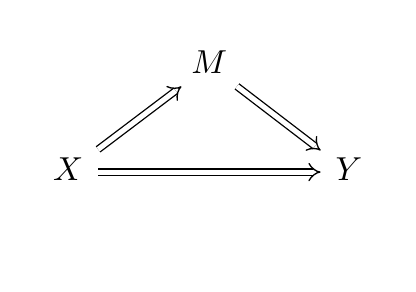
\begin{tikzpicture}[baseline = (a).base]
\node[scale = 1.2] (a) at (0,0){
\begin{tikzcd}[arrows = Rightarrow]
& M \ar[dr] & \\
X \ar[ur] \arrow{rr} & & Y \\
\end{tikzcd}
};
\end{tikzpicture}
\end{center}

where $X_i$ is \emph{rural inequality}, $Y_i$ is the adoption of income tax as the dependent variable of interest, and $M_i$ is \emph{franchise} as the mediator variable. Causal mediation analysis estimates the effect of the independent variable of interest, through an intervening variable - called the mediator. Imai et al (2011) suggest that mediation analysis should be done through the estimation of two equations, which are then simulated together for estimating the average causal mediation effect. The first equation is: 
\begin{align}
M_i = \alpha_1 + \lambda_1 X_i + C \beta + \epsilon_{i1}
\end{align}

Due to the continuous nature of the mediator variable in question, franchise, this takes the form of a least-squares regression in which the left-hand-side variable is \emph{franchise} $(M_i)$ as a function of \emph{rural inequality} $(X_i)$, plus a matrix of control variables from the original model ($C$). The first condition of a causal mediation analysis is that the independent variable will produce a significant effect on the mediator variable. 

The second condition, as demonstrated in the equation below, has the \emph{adoption of the income tax}, $Y_i$ on the left-hand-side, and both the independent variable of interest, \emph{rural inequality} and the mediator, \emph{franchise} on the right-hand-side, along with the same set of controls, $C$ from the original model. 
\begin{align}
Y_i = \alpha_2 + \lambda_2X_i + \gamma M_i + C\beta + \epsilon_{i2}
\end{align}

This second equation takes the form of a logistic regression due to the dichotomous nature of the income tax adoption variable, $Y_i$. In this second condition for a causal mediation analysis, the mediator variable should continue to have a significant effect on the dependent variable, even when controlling for the independent variable of interest. In fact, the more closely related the mediator variable is to the independent variable of interest, we might expect that in a traditional regression, the mediator will absorb the effect of the independent variable of interest when included in the same regression. In part, this resembles the results derived earlier in Table 2 when we compare the effects of including franchise in model 4 to model 3, which does not include franchise.

Finally, using these two equations, the average causal mediation effect (ACME) can be calculated by estimating the effect of \emph{rural inequality}, $X_i$ on the \emph{adoption of income tax}, $Y_i$, through the mediator variable \emph{franchise}, $M_i$. By comparing the average differences in the outcome variable between using $M-_i$ to predict the outcome variable $Y_i$ and the actual model, one can derive the ACME. 

\pagebreak

\subsection{Causal Mediation Results}\hfill\\

In table 4, we present the results of the mediation analyses using model 5 as the basis of comparison. The results have been estimated using nonparametric bootstrap over 1000 simulations, and the main parameter estimates of interest are shaded in grey. The model suggests that \emph{rural inequality} has a negative but statistically significant effect on \emph{franchise}; higher levels of rural inequality is strongly correlated with less of the population participating in the presidential vote. 

From the second model in Table 4, franchise as a mediator asserts a negative and statistically significant effect on the probability of adopting the income tax. Finally, and most importantly, the ACME is negative (estimated at -.0169) and is statistically significant at the 5\% level; Figure 3 shows that 95\% confidence interval is just shy of crossing zero. Since the total effect of rural inequality is estimated to be -0.0428, around 39\% of the total effect is mediated through franchise. This leads us to believe that an important part of inequality negatively influencing the probability of adopting the income tax works through the extension- or exclusion- of franchise.

% Reading mediation results: the total effect is equal to beta_1: the total effect of X on Y without M. 

%The direct effect (ADE) is beta_4 in the third step: a diect effect of X on Y after taking into account a mediation (indirect effect of M). 

% Finally the mediation effect (ACME) is the total effect minus the direct effect (beta_1 - beta_4) which equals to a product of a coefficient of X in the second step and a coefficient of M in the last step (also beta_2 * beta_3)

\begin{table}[!htbp] \centering 
	\caption{Mediation Analysis Results} 
	\label{} 
	\begin{tabular}{@{\extracolsep{5pt}}lcc} 
		\\[-1.8ex]\hline 
		\hline \\[-1.8ex] 
		& \multicolumn{2}{c}{\textit{Dependent variable:}} \\ 
		\cline{2-3} 
		\\[-1.8ex] & franchise\_suffrage & income\_tax \\ 
		\\[-1.8ex] & \textit{OLS} & \textit{logistic} \\ 
		\\[-1.8ex] & (1) & (2)\\ 
		\hline \\[-1.8ex] 
		Franchise &  & {\cellcolor{gray!30}$-$4.407$^{**}$} \\ 
		&  & {\cellcolor{gray!30}(1.899)} \\ 
		& & \\ 
		Rural Inequality & {\cellcolor{gray!30}$-$0.120$^{**}$}& $-$73.267$^{**}$ \\ 
		& {\cellcolor{gray!30}(0.050)} & (32.512) \\ 
		& & \\ 
		Ln(Population) & $-$0.002 & 0.739$^{*}$ \\ 
		& (0.004) & (0.448) \\ 
		& & \\ 
		Ln(GDP) & 0.054$^{***}$ & $-$1.735$^{*}$ \\ 
		& (0.012) & (0.926) \\ 
		& & \\ 
		Urbanization & $-$0.097$^{***}$ & $-$4.965$^{**}$ \\ 
		& (0.021) & (1.954) \\ 
		& & \\ 
		Depression & 0.077$^{***}$ & 1.948$^{***}$ \\ 
		& (0.007) & (0.619) \\ 
		& & \\ 
		War & $-$0.015$^{**}$ & 0.753 \\ 
		& (0.006) & (0.470) \\ 
		& & \\ 
		Racial Heterogeneity & $-$0.305$^{***}$ & $-$0.751 \\ 
		& (0.018) & (1.798) \\ 
		& & \\ 
		Rural Inequality*Franchise &  & 93.004$^{**}$ \\ 
		&  & (46.022) \\ 
		& & \\ 
		\hline \\[-1.8ex] 
		ACME & \multicolumn{2}{c}{\cellcolor{gray!30}-.0167**}  \\ 
		\relax[95\% confidence interval] & \multicolumn{2}{c}{\cellcolor{gray!30}[-.0896, 0.00]} \\ 
		Direct effect & \multicolumn{2}{c}{-.0651**}  \\ 
		\relax[95\% confidence interval] & \multicolumn{2}{c}{[-.186, -.000]}  \\ 
		Total effect & \multicolumn{2}{c}{-.0428**}  \\ 
		\relax[95\% confidence interval] & \multicolumn{2}{c}{[-.115, .01]}  \\ 
		Fixed Effects: & Sub-regional & Sub-regional \\ 
		Observations & 2,090 & 2,090 \\ 
		\hline 
		\hline \\[-1.8ex] 
		\textit{Note:}  & \multicolumn{2}{r}{$^{*}$p$<$0.1; $^{**}$p$<$0.05; $^{***}$p$<$0.01} \\ 
	\end{tabular} 
\end{table} 

\pagebreak

Figure 3 illustrates the effect of the causal mediation graphically. It shows the ACME, direct effect (ADE) and total effect of rural inequality all have a negative effect on the adoption of the income tax and are statistically significant at the 10\% level. The black lines illustrate the non-zero effects of the variables, while the white lines are merely the base reference points for the model.

From this analysis, we can conclude that there is evidence to support \emph{Hypothesis 6}. We believe that rural inequality primarily operates on the adoption of the income tax at least partially through the mechanism of disenfranchisement. Franchise primarily as a mechanism, rather than a causal driver itself is an area that requires further study. This relates well with our final logistic model presented in table 3. While we can see that rural inequality remains statistically significant, we can see that its impact varies greatly at differing levels of franchise in Figure 2. While it makes sense that restrictions on franchise allow for those with franchise to better exercise their preferences around taxation, it is unclear how franchise or lack thereof drives preferences. Further research should be done to understand how the extension, revocation and restriction of franchise plays a roll in all political bargaining and how it mediates preferences across various class cleavages.


\includegraphics[scale=0.80]{ps745-figure2b}

\section{Robustness Checks}

This section will both examine a scaled down version of the model to test to see if the results hold as we narrow in on our parameters of interest. Then we will proceed to expand out to understand if the model is robust to alternate specifications and the inclusion of additional possible confounding variables. We find that the model proves to be fairly resilient and demonstrate that the core variables of interest remain relatively unchanged by the inclusion of additional variables.

\subsection{Scaled Down}

We present here a scaled down version of model 5- after introducing the control for Secession. In this model- presented in Table 5- we remove all variables outside of \emph{Rural Inequality}, \emph{Franchise}, \emph{Depression}, and \emph{Urbanization} then proceed to run the model along with our Sub-Regional and Secession controls. 

\begin{table}[!htbp] \centering 
	\caption{The Adoption of the Income Tax as a function of Inequality and Franchise} 
	\label{} 
	\begin{tabular}{@{\extracolsep{5pt}}lccc} 
		\\[-1.8ex]\hline 
		\hline \\[-1.8ex] 
		& \multicolumn{3}{c}{\textit{Dependent variable:}} \\ 
		\cline{2-4} 
		\\[-1.8ex] & \multicolumn{3}{c}{Income Tax Adoption} \\ 
		\\[-1.8ex] & (1) & (2) & (3)\\ 
		\hline \\[-1.8ex] 
		Rural Inequality & $-$73.267$^{**}$ & $-$72.276$^{**}$ & $-$45.491$^{**}$ \\ 
		& (32.512) & (32.600) & (21.861) \\ 
		Franchise & $-$4.407$^{**}$ & $-$7.358$^{***}$ & $-$6.703$^{***}$ \\ 
		& (1.899) & (2.279) & (2.135) \\ 
		Ln(Population) & 0.739$^{*}$ &  &  \\ 
		& (0.448) &  &  \\ 
		Ln(GDP) & $-$1.735$^{*}$ &  &  \\ 
		& (0.926) &  &  \\ 
		Urbanization & $-$4.965$^{**}$ & $-$5.988$^{***}$ & $-$5.134$^{***}$ \\ 
		& (1.954) & (1.502) & (1.246) \\ 
		Great Depression & 1.948$^{***}$ & 2.251$^{***}$ & 2.136$^{***}$ \\ 
		& (0.619) & (0.546) & (0.527) \\ 
		War & 0.753 &  &  \\ 
		& (0.470) &  &  \\ 
		Racial Heterogeneity & $-$0.751 &  &  \\ 
		& (1.798) &  &  \\ 
		Rural*Franchise & 93.004$^{**}$ & 86.931$^{*}$ & 54.285$^{*}$ \\ 
		& (46.022) & (45.350) & (32.247) \\ 
		Constant & $-$1.151 & $-$2.864 & $-$3.351$^{*}$ \\ 
		& (9.183) & (2.052) & (1.714) \\ 
		\hline \\[-1.8ex] 
		Fixed Effects: & Sub-regional & Sub-regional & No \\ 
		Observations & 2,090 & 2,090 & 2,090 \\ 
		Log Likelihood & $-$157.342 & $-$159.773 & $-$162.190 \\ 
		Akaike Inf. Crit. & 356.684 & 355.547 & 344.381 \\ 
		\hline 
		\hline \\[-1.8ex] 
		\textit{Note:}  & \multicolumn{3}{r}{$^{*}$p$<$0.1; $^{**}$p$<$0.05; $^{***}$p$<$0.01} \\ 
	\end{tabular} 
\end{table}  

As can be seen in the table, there is change in the variables of interest, but they maintain their relative magnitude and direction. To check if our results still hold, we graph the variables similarly to how we had done in Figure 1. This graph is presented in Figure 4, now with confidence intervals included. As can be seen, the effects of the plots are still similar to those in Figure 1. Unfortunately, the data is fairly unstable due to regional effects, so the confidence intervals obstruct the analysis and call into question the extent the relationship is robust. To try and eliminate some of the uncertainty, we remove the sub-regional controls and run the model again. This is model 3 in Table 5.

\includegraphics[scale=1]{ps745-figure4}


 As can be seen, the directions remain unchanged in the model, but the magnitudes of several of the variables have changed noticeably. Most noticeably, of our three main variables of interest, all have remained significant except for the interaction. To see if the confidence interval analysis has stabilized, we rerun Figure 4 and present it below as Figure 5. Unfortunately, it is easily apparent that there is still inherent instability related to the model that creates large confidence intervals. While we remain confident that our hypotheses remain viable, these results are concerning and merit further examination. We are reasonably confident that our model remains robust to the removal of controls based on this quick analysis and believe that there is no evidence to revise any of our hypotheses based on the analysis of scaled down versions of our model.
 
 \includegraphics[scale=01]{ps745-figure5}
 
 
 \subsection{Extensions of the Model}
 
 In this section we will check the robustness of our results to the inclusion of different confounding variables. We will present several alternative specifications of the model that include variables that could confound our hypotheses. We find that our model remains fairly robust to these alternative specifications. We begin with Table 6. Our first step is to compare the original final model in column 1 vs the model where we control for secession. While this does lead to a magnitude change in our three key variables of interest (\emph{Rural Inequality}, \emph{Franchise}, and the interaction), the signs and their statistical significance remain unchanged. It is interesting to note that inclusion in the group of states that seceded from the Union during the American Civil War does lead to a statistically significant decrease in the odds of adoption of the income tax. We move into the 3rd column of Table 6 by controlling for the pre-Great Depression era. This variable is statistically insignificant, and also creates insignificance for our Great Depression control, but again our 3 key variables of interest remain relatively unchanged. Pursuing an alternative hypothesis- that rather than measuring family farms for rural inequality, we should look at the importance the largest of farms, we introduce a variable to control for what percentage of farms within a state match the definition of large farms (greater than 1,000 acres). Inclusion of this variable is negative and statistically significant, but the magnitude of our other three variables (while maintaining their significance) has increased and the net effect does little to change our hypotheses that agrarian elites actually had little to do with the adoption of the income tax, and instead the story should focus on middle class agrarians.
 
 \begin{table}[!htbp] \centering 
 	\caption{The Adoption of the Income Tax as a function of Inequality and Franchise} 
 	\label{} 
 	\begin{tabular}{@{\extracolsep{5pt}}lcccc} 
 		\\[-1.8ex]\hline 
 		\hline \\[-1.8ex] 
 		& \multicolumn{4}{c}{\textit{Dependent variable:}} \\ 
 		\cline{2-5} 
 		\\[-1.8ex] & \multicolumn{4}{c}{Income Tax Adoption} \\ 
 		\\[-1.8ex] & (1) & (2) & (3) & (4)\\ 
 		\hline \\[-1.8ex] 
 		Rural Inequality & $-$73.267$^{**}$ & $-$83.598$^{**}$ & $-$83.748$^{**}$ & $-$80.023$^{**}$ \\ 
 		& (32.512) & (33.836) & (33.870) & (34.838) \\ 
 		Franchise & $-$4.407$^{**}$ & $-$8.666$^{***}$ & $-$8.633$^{***}$ & $-$10.452$^{***}$ \\ 
 		& (1.899) & (2.504) & (2.510) & (2.602) \\ 
 		Ln(Population) & 0.739$^{*}$ & 1.050$^{**}$ & 1.050$^{**}$ & 1.095$^{**}$ \\ 
 		& (0.448) & (0.481) & (0.481) & (0.482) \\ 
 		Ln(GDP) & $-$1.735$^{*}$ & $-$2.538$^{***}$ & $-$2.544$^{***}$ & $-$1.967$^{**}$ \\ 
 		& (0.926) & (0.970) & (0.970) & (0.979) \\ 
 		Urbanization & $-$4.965$^{**}$ & $-$4.056$^{**}$ & $-$4.054$^{**}$ & $-$3.365$^{*}$ \\ 
 		& (1.954) & (1.888) & (1.889) & (1.879) \\ 
 		Great Depression & 1.948$^{***}$ & 1.929$^{***}$ & 1.706 & 2.102$^{***}$ \\ 
 		& (0.619) & (0.654) & (1.510) & (0.653) \\ 
 		War & 0.753 & 0.687 & 0.691 & 0.541 \\ 
 		& (0.470) & (0.477) & (0.478) & (0.497) \\ 
 		Racial Heterogeneity & $-$0.751 & 0.534 & 0.541 & $-$0.050 \\ 
 		& (1.798) & (1.768) & (1.768) & (1.826) \\ 
 		Secession &  & $-$3.317$^{***}$ & $-$3.306$^{***}$ & $-$3.484$^{***}$ \\ 
 		&  & (1.165) & (1.166) & (1.132) \\ 
 		Pre-Great Depression &  &  & $-$0.325 &  \\ 
 		&  &  & (1.982) &  \\ 
 		Percent of Large Farms &  &  &  & $-$19.657$^{**}$ \\ 
 		&  &  &  & (8.536) \\ 
 		Rural*Franchise & 93.004$^{**}$ & 112.179$^{**}$ & 112.429$^{**}$ & 152.223$^{***}$ \\ 
 		& (46.022) & (47.697) & (47.758) & (51.199) \\ 
 		Constant & $-$1.151 & 1.573 & 1.868 & $-$2.974 \\ 
 		& (9.183) & (9.419) & (9.591) & (9.906) \\ 
 		\hline \\[-1.8ex] 
 		Fixed Effects: & Sub-regional & Sub-regional & Sub-regional & Sub-regional \\ 
 		Observations & 2,090 & 2,090 & 2,090 & 2,090 \\ 
 		Log Likelihood & $-$157.342 & $-$153.392 & $-$153.378 & $-$149.487 \\ 
 		Akaike Inf. Crit. & 356.684 & 350.784 & 352.757 & 344.974 \\ 
 		\hline 
 		\hline \\[-1.8ex] 
 		\textit{Note:}  & \multicolumn{4}{r}{$^{*}$p$<$0.1; $^{**}$p$<$0.05; $^{***}$p$<$0.01} \\ 
 	\end{tabular} 
 \end{table}
 
 Moving forward, we present Table 7. Column 1 maintains for comparison our final model from section 5 and continues to build on our models in Table 6. Column 2 introduces an interaction between top farms and franchise, which perhaps unsurprisingly does lead to a loss of significance for all of our variables except for 
\emph{franchise}. Instead of building upon this model further, we instead turn to an alternative hypothesis- that it is not the number of farms that are below a certain size that matter, but rather the number of farms that are operated by the family that owns them- rather than being corporations or tenant farms for example. This is presented in column 3. The inclusion of this variable does affect changes in our variables of interest. While we lose significance in our variables of interest, we argue that this is due to the significant overlap between the variables of family farms (defined as farms less than 500 acres) and family owned and operated farms. This creates a large amount of variance in the data as multicollinearity increases. An interesting effect is observed in column 4 when we interact the family owned farms with Franchise. We regain significance on both \emph{rural inequality} and the interaction with \emph{franchise}, while simultaneously adding significance to family owned farms and it's interaction with Franchise. The change of magnitude on the original interaction is statistically significant, but has actually increased the effect. The net total effect suggests that our hypothesis of placing heightened emphasis on middle class agrarians is a correct restructuring of the narrative around income tax adoption away from agrarian elites.

\begin{table}[!htbp] \centering 
	\caption{The Adoption of the Income Tax as a function of Inequality and Franchise} 
	\label{} 
	\begin{tabular}{@{\extracolsep{5pt}}lcccc} 
		\\[-1.8ex]\hline 
		\hline \\[-1.8ex] 
		& \multicolumn{4}{c}{\textit{Dependent variable:}} \\ 
		\cline{2-5} 
		\\[-1.8ex] & \multicolumn{4}{c}{Income Tax Adoption} \\ 
		\\[-1.8ex] & (1) & (2) & (3) & (4)\\ 
		\hline \\[-1.8ex] 
		Rural Inequality & $-$73.267$^{**}$ & $-$6.942 & $-$86.843$^{**}$ & $-$87.220$^{**}$ \\ 
		& (32.512) & (90.724) & (34.476) & (34.208) \\ 
		Franchise & $-$4.407$^{**}$ & $-$10.361$^{***}$ & $-$8.790$^{***}$ & 3.093 \\ 
		& (1.899) & (2.623) & (2.527) & (4.963) \\ 
		Ln(Population) & 0.739$^{*}$ & 1.113$^{**}$ & 1.032$^{**}$ & 1.106$^{**}$ \\ 
		& (0.448) & (0.492) & (0.475) & (0.483) \\ 
		Ln(GDP) & $-$1.735$^{*}$ & $-$1.960$^{*}$ & $-$2.562$^{***}$ & $-$2.684$^{***}$ \\ 
		& (0.926) & (1.002) & (0.968) & (0.968) \\ 
		Urbanization & $-$4.965$^{**}$ & $-$2.903 & $-$4.043$^{**}$ & $-$4.395$^{**}$ \\ 
		& (1.954) & (1.977) & (1.863) & (1.915) \\ 
		Great Depression & 1.948$^{***}$ & 2.139$^{***}$ & 1.867$^{***}$ & 1.760$^{**}$ \\ 
		& (0.619) & (0.656) & (0.666) & (0.687) \\ 
		War & 0.753 & 0.548 & 0.717 & 0.735 \\ 
		& (0.470) & (0.498) & (0.483) & (0.487) \\ 
		Racial Heterogeneity & $-$0.751 & $-$0.106 & 0.433 & 0.608 \\ 
		& (1.798) & (1.835) & (1.799) & (1.752) \\ 
		Secession &  & $-$3.432$^{***}$ & $-$3.500$^{***}$ & $-$3.144$^{***}$ \\ 
		&  & (1.141) & (1.184) & (1.163) \\ 
		Percent of Large Farms &  & $-$65.418 &  &  \\ 
		&  & (56.644) &  &  \\ 
		Percent of Family
		Owned/Operated &  &  & $-$1.201 & 9.561$^{**}$ \\ 
		&  &  & (1.258) & (4.173) \\ 
		Rural*Franchise & 93.004$^{**}$ & 38.917 & 117.138$^{**}$ & 118.512$^{**}$ \\ 
		& (46.022) & (134.115) & (48.531) & (48.248) \\ 
		Top Farms*Franchise &  & 70.490 &  &  \\ 
		&  & (81.569) &  &  \\ 
		Own Farms*Franchise &  &  &  & $-$18.330$^{***}$ \\ 
		&  &  &  & (6.673) \\ 
		Constant & $-$1.151 & $-$3.527 & 2.976 & $-$4.800 \\ 
		& (9.183) & (10.308) & (9.501) & (9.838) \\ 
		\hline \\[-1.8ex] 
		Fixed Effects: & Sub-regional & Sub-regional & Sub-regional & Sub-regional \\ 
		Observations & 2,090 & 2,090 & 2,090 & 2,090 \\ 
		Log Likelihood & $-$157.342 & $-$149.008 & $-$152.972 & $-$149.306 \\ 
		Akaike Inf. Crit. & 356.684 & 346.016 & 351.944 & 346.611 \\ 
		\hline 
		\hline \\[-1.8ex] 
		\textit{Note:}  & \multicolumn{4}{r}{$^{*}$p$<$0.1; $^{**}$p$<$0.05; $^{***}$p$<$0.01} \\ 
	\end{tabular} 
\end{table} 
 
 To conclude our robustness checks, we test our model against two additional plausible explanations for preferences for redistribution- the level of income and the percent of the population that is female. Both of these have been proposed as affecting preferences for redistribution and therefore- by logical extension- preferences for taxation. Table 8 presents our original model in column 1. Column 2 includes a control for levels of GDP. While we lack measures of inequality in our data related to income, by testing levels of total income within a state both against itself in the future and against other states within the same time period, we believe this should show some effect if income per capita is a significant factor in the model. We find that the inclusion of state income per capita has only a marginal affect on the magnitude of our variables of interest (increasing them), and no affect on statistical significance. Nor does the variable take on significance of its own. Column 3 includes a further control to account for the percentage of the population that is female. Again we find no affect on the variables of interest and this variable fails to take on any statistical significance.
 
\begin{table}[!htbp] \centering 
	\caption{The Adoption of the Income Tax as a function of Inequality and Franchise} 
	\label{} 
	\begin{tabular}{@{\extracolsep{5pt}}lccc} 
		\\[-1.8ex]\hline 
		\hline \\[-1.8ex] 
		& \multicolumn{3}{c}{\textit{Dependent variable:}} \\ 
		\cline{2-4} 
		\\[-1.8ex] & \multicolumn{3}{c}{Income Tax Adoption} \\ 
		\\[-1.8ex] & (1) & (2) & (3)\\ 
		\hline \\[-1.8ex] 
		Rural Inequality & $-$73.267$^{**}$ & $-$83.952$^{**}$ & $-$80.771$^{**}$ \\ 
		& (32.512) & (33.791) & (34.711) \\ 
		Franchise & $-$4.407$^{**}$ & $-$8.682$^{***}$ & $-$8.697$^{***}$ \\ 
		& (1.899) & (2.498) & (2.514) \\ 
		State Income per Capita &  & $-$0.0001 & $-$0.0001 \\ 
		&  & (0.0002) & (0.0002) \\ 
		Female Population Percent &  &  & 9.805 \\ 
		&  &  & (28.918) \\ 
		Ln(Population) & 0.739$^{*}$ & 1.033$^{**}$ & 0.958$^{*}$ \\ 
		& (0.448) & (0.485) & (0.531) \\ 
		Ln(GDP) & $-$1.735$^{*}$ & $-$2.252 & $-$2.179 \\ 
		& (0.926) & (1.420) & (1.449) \\ 
		Urbanization & $-$4.965$^{**}$ & $-$3.970$^{**}$ & $-$4.107$^{**}$ \\ 
		& (1.954) & (1.916) & (1.951) \\ 
		Great Depression & 1.948$^{***}$ & 1.923$^{***}$ & 1.934$^{***}$ \\ 
		& (0.619) & (0.655) & (0.653) \\ 
		War & 0.753 & 0.696 & 0.700 \\ 
		& (0.470) & (0.478) & (0.478) \\ 
		Racial Heterogeneity & $-$0.751 & 0.534 & 0.439 \\ 
		& (1.798) & (1.763) & (1.791) \\ 
		Secession &  & $-$3.290$^{***}$ & $-$3.389$^{***}$ \\ 
		&  & (1.166) & (1.212) \\ 
		Rural*Franchise & 93.004$^{**}$ & 112.222$^{**}$ & 107.098$^{**}$ \\ 
		& (46.022) & (47.584) & (49.404) \\ 
		Constant & $-$1.151 & $-$0.253 & $-$4.351 \\ 
		& (9.183) & (11.545) & (16.765) \\ 
		\hline \\[-1.8ex] 
		Fixed Effects: & Sub-regional & Sub-regional & Sub-Regional \\ 
		Observations & 2,090 & 2,090 & 2,090 \\ 
		Log Likelihood & $-$157.342 & $-$153.353 & $-$153.295 \\ 
		Akaike Inf. Crit. & 356.684 & 352.706 & 354.589 \\ 
		\hline 
		\hline \\[-1.8ex] 
		\textit{Note:}  & \multicolumn{3}{r}{$^{*}$p$<$0.1; $^{**}$p$<$0.05; $^{***}$p$<$0.01} \\ 
	\end{tabular} 
\end{table}


This robustness section serves to help solidify our confidence in our results. We have attempted to test the extent to which our model holds up under alternative assumptions and specifications within the limits of our data and have found the results to be reasonably robust. At no point in our robustness analysis did we find a change in the sign- either statistically significant or not- of our key variables of interest, nor did we find any evidence to suggest that our hypotheses should be rejected. The robustness checks were not all positive however- we do find graphing our effects that the confidence intervals remain too large for us to make definitive statements, and is definitely an area for future exploration.

\pagebreak

\section{Conclusion}

In examining the case of income tax adoption in the United States, this paper has demonstrated that despite the precedence set by the federal government, subnational adoption is governed by complex dynamics that involve bargaining between myriad sectors of society. These laws are seemingly subordinate primarily to the interests of elites- until an economic imperative as significant as the Great Depression requires the state to bolster its revenue intake. This paper seeks to explain why the general characterization of the adoption of the income tax being positively correlated with the extensive power of an agrarian elite, as seems to be the case in Europe, is not applicable in the case of the United States- at least at the subnational level. 

While existing explanations privilege external influences- such as war- as drivers behind the development of the fiscal state, these theories are limited in explaining within state variation. Our article re-examines other explanations that advocate for an increased role for political and economic elites, where variance in the distribution of such interests and endowments is more likely at the subnational level. The United States serves as an excellent testing ground for examining the effects of bargaining power due to the heterogeneity of both economic and political factors within states while having somewhat homogenous external shocks. The results suggest that in the United States, the adoption of the income tax was most likely in states with middling levels of rural inequality where neither agricultural nor capitalist elites dominated. 

This paper began by reviewing the somewhat sparse literature around taxation to emphasize the need for examination of the subnational differences that drive state fiscal capacity development. We then provided an overview of the historical instance of income tax adoption at the federal level of the United States and described in brief the various political and economic factors that influenced bargaining power between class cleavages- the Great Depression, the increase of urbanization in many states, and the expansion of franchise being particularly salient. Following this, we developed several hypotheses that challenged the current thinking around the factors that are most likely to influence income tax adoption. Primarily, we challenge the hypothesis asserted in earlier literature that high rural inequality increased the probability of income tax adoption. 

Indeed, we find that high levels of rural inequality within the US decreases the probability of adoption compared to middle levels. We also show evidence that demonstrates that extreme shocks to funding for state expenditure can create situations that encourage the adoption of more sophisticated taxation; the Great Depression as a factor proved incredibly robust and is positively correlated with adoption. Despite this, we do in fact find evidence to support the notion that capitalist elites prove resistant to income tax adoption; urbanization- one measure of the strength of non-agrarian industry- is consistently negative with the rate of adoption. Finally, we show evidence that supports the hypothesis concerning the importance of disenfranchisement in accomplishing the adoption of the income tax- however, the evidence we find suggests that rather than being causal in and of itself, disenfranchisement serves as a mechanism by which rural inequality impacts the adoption of an income tax at the subnational level.

Our account advocates that examining the adoption of the income tax in isolation at the national level, without considering the plethora of subnational conditions related to its adoption, is likely to overlook crucial factors related to the bargaining process. Ignoring other considerations that elites may be entertaining when they choose to actively campaign against (or for) its adoption can create misleading conclusions that overemphasize external factors. Additionally, the results seem to strengthen the argument that existing models of redistribution overemphasize the role of preferences for taxation at the expense of analyzing the role of elite cleavages in situations of limited electoral suffrage (\citealt{mares2015non}; \citealt{ansell2014inequality}; \citealt{aidt2009taxman}). 

This paper is but a brief examination of several plausible hypotheses governing the adoption of income tax at the subnational level, and in but one specific context. The conclusions we make, however offer insight into numerous additional areas that are ripe for study. Indeed, we believe that this paper raises significantly more questions than it answers. Future research should seek to better understand the development of overall state capacity at the subnational level, separate from the federal government. Additionally, we find a need for further work to undertake studying the transition from traditional agrarian elites to post-industrial revolution farming- characterized by corporations and large-scale farms that were made possible by new technology that created increasing returns to scale. 

It is undeniable that the shape of agriculture is changing across America\footnote{Farmers today are both significantly older and a substantially smaller part of the population than they have been at any other time in American history. \citealt{tariffs}}, but understanding how it is changing around the world will be informative in examining the influence of agrarians in future political decision making. Further research is also needed to examine how bargaining between various class cleavages will result in expansion or reduction of taxation in developing economies. By the early 20th century, the United States was already a relatively highly developed economy, and the lessons we observed here may not be insightful in understanding state development in less industrialized societies. Furthermore, the United States, while not unique in its subnational structure, has the benefit of relatively well-defined state structure that lends itself to easy analysis; states with more amorphous borders or less concrete distinction between supranational and national institutions will be more difficult to study, but are plausibly more informative in the context of developing economies.

In our particular sample, we would hope for more concrete evidence that examines income inequality at the state level. We were unable to find measures of median income that covered our whole sample size, and using this type of measure in conjunction with rural inequality might prove more informative about the role of inequality in driving adoption of an income tax. Additionally, it would prove useful to understand state by state distributions of income to prove more informative about the relative strength of a middle class that could be observed directly, rather than posited through conjecture. Additionally, there is a plausible reason to suspect that urbanization and rural inequality overlap in some ways; while we have constructed a unique source to measure rural inequality, we believe that its measurement could be better informed by future research.

\pagebreak

\bibliography{ps745-final}

\end{document}
